\documentclass{standalone}
\usepackage{amsmath}
\usepackage{amssymb}
\usepackage{listings}
\usepackage{tikz}
\usepackage{xcolor}

\usetikzlibrary{calc}
\definecolor{backcolour}{rgb}{0.95,0.95,0.92}
\definecolor{codepurple}{rgb}{0.58,0,0.82}

\begin{document}

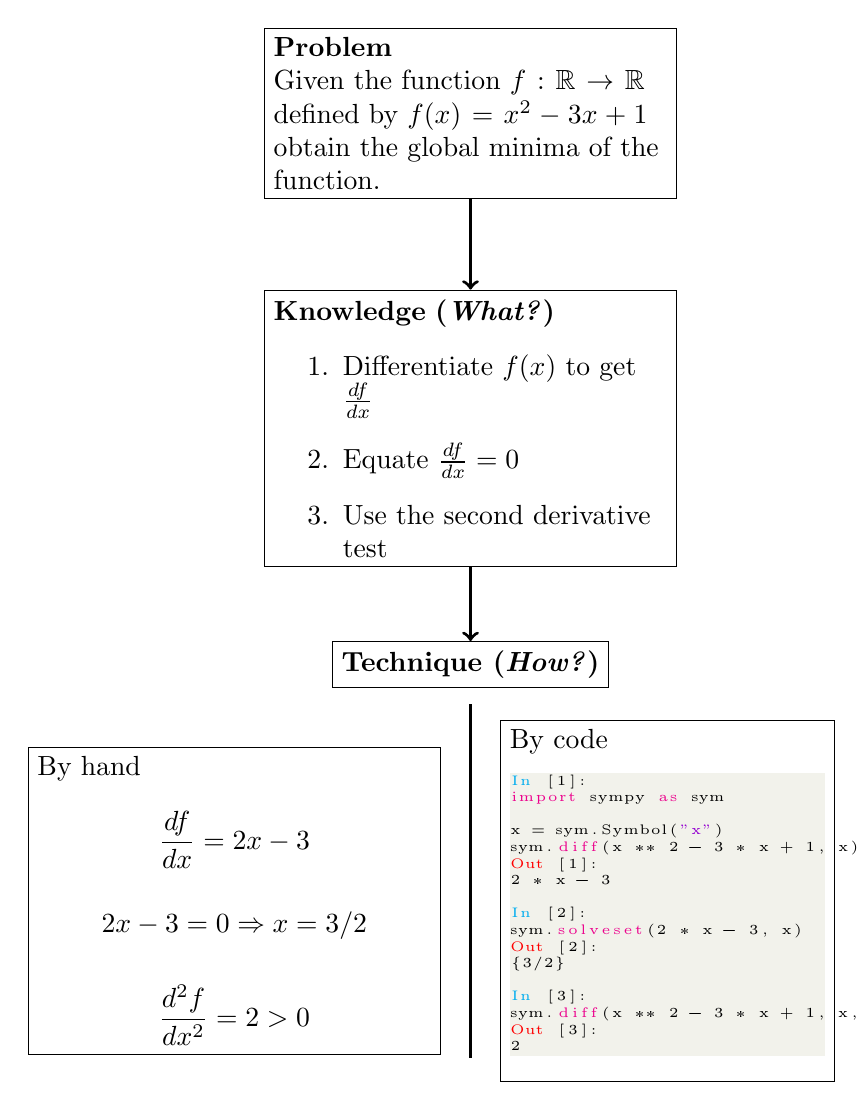
\begin{tikzpicture}
    \node (problem) [draw, text width=5cm] at (0, 0) {\textbf{Problem}

    Given the function \(f:\mathbb{R}\to\mathbb{R}\) defined by \(f(x) = x ^
    2 - 3 x + 1\) obtain the global minima of the function.

    };

    \node (knowledge) [draw, text width=5cm] at ($(problem) + (0, -4)$) {\textbf{Knowledge (\textit{What?})}
        \begin{enumerate}
                \item Differentiate \(f(x)\) to get \(\frac{df}{dx}\)
                \item Equate \(\frac{df}{dx}=0\)
                \item Use the second derivative test 
        \end{enumerate}
    };

    \draw [very thick, ->] (problem) -- (knowledge);

    \node (technique) [draw] at ($(knowledge) + (0, -3)$) {\textbf{Technique (\textit{How?})}};
    \draw [very thick, ->] (knowledge) -- (technique);
    \draw [very thick] ($(knowledge) + (0, -3.5)$) -- ($(knowledge) + (0, -8)$);

    \node (by_hand) [draw, text width=5cm] at ($(technique) + (-3, -3)$) {By hand
    
    \[\frac{df}{dx} = 2 x - 3\]

    \[2x-3 =0 \Rightarrow x = 3/2\]

    \[\frac{d^2f}{dx^2} = 2 > 0\]
    };


\lstset{backgroundcolor=\color{backcolour}}
\lstset{keywordstyle=\color{magenta}}
\lstset{keywordstyle=[2]\color{cyan}}
\lstset{keywordstyle=[3]\color{red}}
\lstset{stringstyle=\color{codepurple}}
\lstset{language=Python}
\lstset{morekeywords={diff, solveset}}
\lstset{keywords=[2]{In}}
\lstset{keywords=[3]{Out}}
    \node (code) [draw, text width=4cm] at ($(technique) + (2.5, -3)$) {By code
\tiny
\begin{lstlisting}
In [1]:
import sympy as sym

x = sym.Symbol("x")
sym.diff(x ** 2 - 3 * x + 1, x)
Out [1]:
2 * x - 3

In [2]:
sym.solveset(2 * x - 3, x)
Out [2]:
{3/2}

In [3]:
sym.diff(x ** 2 - 3 * x + 1, x, 2)
Out [3]:
2
\end{lstlisting}
    };


\end{tikzpicture}
\end{document} 
